\section{Methodology (deprecated)}

{\color{blue} In this section we should go straight to our method introducing al the ingredients described in Alg 1 .. 

}


{\color{blue}
This 1st paragraph is more related with the Introduction section ...
}
\\
Watermarking for diffusion models generally consists of two fundamental phases: \textit{injection} and \textit{verification}. 
Diffusion-based generative models have become central to modern content creation, raising the need for reliable mechanisms to identify and verify AI-generated content. Watermarking serves as a key strategy to ensure content authenticity and model accountability, particularly for pretrained diffusion models that are already widely deployed by technology providers. A well-designed watermarking system enables the model owner to prove that an image originates from their generative model while preserving image quality and generation performance.

In this work, we formalise the complete watermarking workflow as a unified pipeline comprising watermark injection, verifier dataset construction, and probabilistic verification, as summarised in Algorithm~\ref{alg:overall_pipeline}. Specifically, a fixed frequency-domain watermark is injected at the noise level prior to image generation, ensuring compatibility with pretrained diffusion models without modifying their weights. To enable robust verification, we construct a dedicated verifier dataset by generating paired unwatermarked and watermarked images under identical prompts and noise initialisations, from which frequency-domain features are extracted to train a lightweight verifier. At inference time, the trained verifier outputs a calibrated watermark confidence score for a given image, allowing reliable detection under a fixed operating threshold.



\begin{figure*}
    \centering
    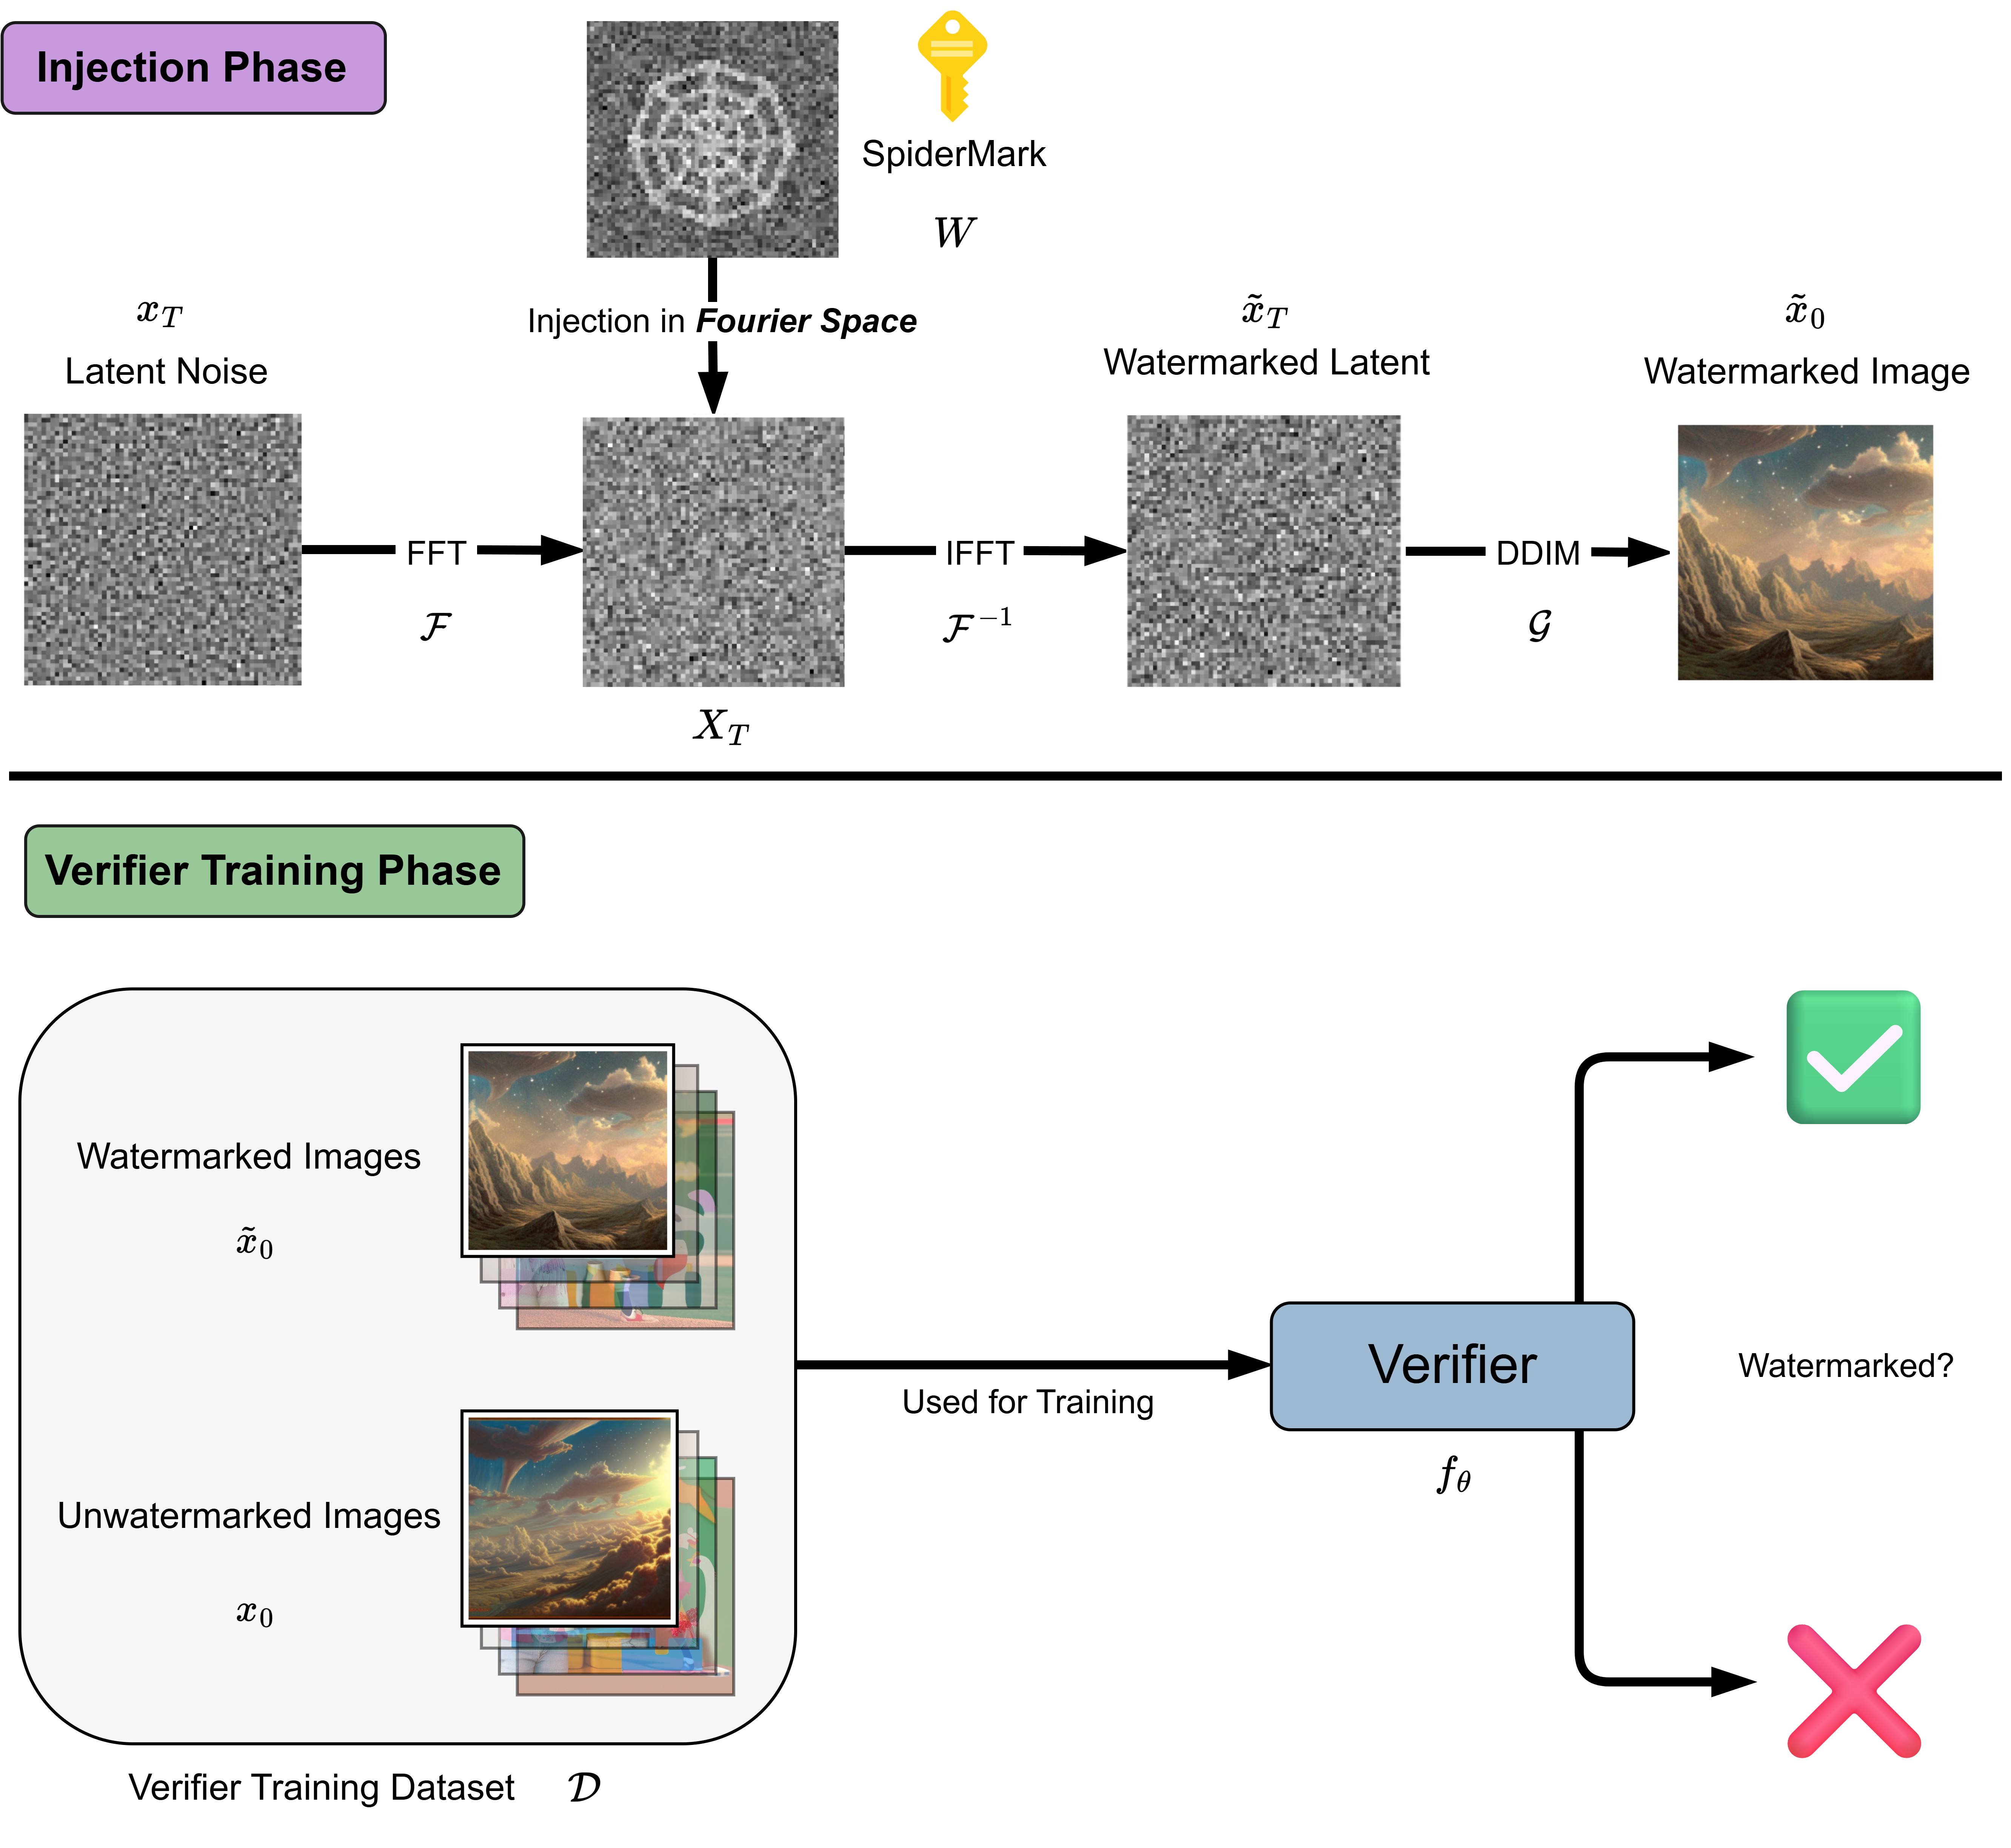
\includegraphics[width=.9\linewidth]{figures/spidernet-overview.png}
    \caption{Overview of the proposed SpiderMark watermarking framework.
\textbf{Top}: Injection phase, where a fixed SpiderMark pattern is injected into the initial diffusion noise in the Fourier domain before DDIM sampling, producing a watermarked image without modifying the pretrained model.
\textbf{Bottom}: Verifier training and inference, where paired watermarked and unwatermarked images are used to train a verifier that outputs a probabilistic watermark confidence at test time.}
    \label{fig:spidernet}
\end{figure*}



{\color{blue} This paragraph is suited for the related work. We could add this class of diffusion base models. I did not move yet this part to the related work section}

\paragraph{Watermarking Strategies in Diffusion Models.}
Diffusion watermarking techniques can generally be divided into two categories: progressive injection and direct noise-level injection. 
The first, progressive injection, embeds watermark information gradually across the denoising trajectory. 
In this approach, watermark signals are added to intermediate representations \(x_t\) at multiple timesteps, influencing the generative process across varying noise levels. 
While this method allows fine-grained control, it requires modifying the sampling process or accessing model weights, often reducing visual quality and computational efficiency.

In contrast, direct noise-level injection introduces the watermark once into the initial Gaussian noise tensor \(x_T\) before denoising begins. 
This approach does not require any architectural or algorithmic changes, making it suitable for pretrained diffusion models. 
By injecting the watermark at the earliest stage, the pattern propagates naturally through the reverse diffusion process and emerges in the final image \(x_0\) as a stable, spectral signature. 
SpiderMark adopts this direct injection paradigm, offering a practical solution for existing diffusion models deployed by technology companies that seek to add watermarking without retraining their models.
